% !TEX root=../master.tex
\chapter{Introduction}
\label{ch:introduction}

% Brainstorming:
% \begin{itemize}
%     \item Moving Target Handoff for Perpetual Tracking in GPS-Denied Environments
%     \item Moving target handoff without GPS
%     \item Overcoming UAS limitations through synergistic autonomy
% \end{itemize}
%
% Moving target handoff for perpetual tracking in gps-denied environments:
% \begin{itemize}
%     \item UAVs have limited flight time (gas/battery limitations)
%     \item It is difficult to maintain meaningful information in GPS-denied environments.
%     \item Example: search and rescue scenario
%     \item Example: military applications
% \end{itemize}

\section{Background}
Unmanned aerial systems (UAS) are useful for surveillance and monitoring, utilizing a high vantage point to observe activity on the ground.
Many surveillance and monitoring applications make use of small unmanned aerial systems (sUAS) which are relatively inexpensive, agile, and easy to deploy.
These smaller vehicles, however, often have a limited fuel or battery capacity and cannot operate for extended periods of time.
The limited flight time makes it difficult for a single sUAS to persistently track or monitor ground activity.
This issue can be overcome by utilizing multiple vehicles to cooperatively monitor an area, while sharing global information between the vehicles or with a central station, such as in \cite{WatsonCoutoSussman18,ValentiDaleHowFariasVian12}.
While these types of multi-agent approaches are effective, they typically rely upon GPS to coordinate locations and information.
GPS signals are not always reliable and can even be susceptible to jamming and spoofing~\cite{KernsShepardBhattiHumphreys2014}.
Accordingly, solutions that are independent of GPS can allow for unhindered operation in a wider variety of situations.
This work focuses on providing a robust solution for persistent tracking of moving ground targets from fixed-wing UAS without GPS.

The primary difficulty in tracking ground targets for extended periods of time without GPS is the transition or ``handoff'' between two sUAS.
When one vehicle that is tracking a target becomes low on fuel, another vehicle must be deployed to replace the current sUAS without any loss of information.
Enabling this handoff scenario is the primary motivation for this paper.
The UAS that is currently tracking the target of interest is referred to as the ``tracking UAS'' and the oncoming replacement vehicle is referred to as the ``handoff UAS.'' Section~\ref{sec:architecture} gives a summary of the technical challenges involved in the target handoff problem as well as the proposed solutions for each challenge.


\section{Architecture}
\begin{figure}[hbt]
    \centering
    \includegraphics[width=1.0\columnwidth]{figures/intro/handoff_diagram_with_eq1}
    \caption{Diagram of the target handoff problem. The numbers depict the five main components of the handoff problem, 1) self-pose estimation, 2) relative-pose estimation, 3) orbit insertion, 4) target tracking, and 5) the handoff logic. The equation and related symbols depict Equation~\eqref{eq:target_rel_pos}}
    \label{fig:handoff_diagram}
\end{figure}

The fundamental geometric relationship for the handoff problem, shown in Figure~\ref{fig:handoff_diagram}, is given by
        \begin{equation} \label{eq:target_rel_pos}
            \p_{\TGwrtH}^\hb = \Rot{\hv}{\hb}\left(\p_{\TwrtH}^\hv + \Rot{\tv}{\hv}\Rot{\tb}{\tv}\p_{\TGwrtT}^\tb\right),
        \end{equation}
where the objective is to find $\mathbf{p}_{t/h}^{h_b}$, the position of the target relative to the handoff vehicle, in the body frame of the handoff UAS, given $\mathbf{p}_{t/r}^{r_b}$, the position of the target relative to the tracker, expressed in the body frame of the tracking UAS.

The handoff problem can be broken into the following five main parts, as depicted in Figure~\ref{fig:handoff_diagram}.
\begin{enumerate}
    \item \textbf{Self-pose Estimation: }
        Self-pose estimation refers to the estimation of the rotation matrices $R_{r_\ell}^{r_b}$ and $R_{h_\ell}^{h_b}$, which represent the transformation between the local-level frames and the body frames of the tracker and handoff vehicles respectively.  In essence, this requires estimating the roll and pitch angles of each vehicle using only the IMU and pressure sensors.  
    \item \textbf{Relative-pose Estimation: }
        Relative pose estimation is the problem of estimating $\mathbf{p}_{r/h}^{h_\ell}$, the position of the tracker relative to the handoff vehicle, expressed in the local-level frame of the handoff UAS, and $R_{r_\ell}^{h_\ell}$ the transformation from the local-level frame of the tracker to the local-level frame of the handoff UAS.  
    \item \textbf{GPS-denied Orbit Control: }
        Using the estimate of the target's position, the handoff vehicle then inserts itself into a similar orbit about the target.
        Initially the handoff UAS will use the relative line-of-sight (LOS) vector $\mathbf{p}_{t/h}^{h_b}$ to the target from Equation~\eqref{eq:target_rel_pos} to navigate into an orbit about the target. After the handoff process is complete, the handoff vehicle will orbit the target completely based on visual information, independent of measurements from the tracking UAS.
    \item \textbf{Multiple-target Tracking: }
        Once the handoff UAS is in orbit about the target, it utilizes a gimballed camera to track the target.
        There is also the possibility that there are multiple moving objects on the ground, so the tracking algorithm must be capable of simultaneously tracking an arbitrary number of moving targets in real time.  
    \item \textbf{Handoff Logic: }
        When the handoff UAS is successfully tracking moving targets on the ground, it must use information from the tracking UAS to ensure it selects the correct target.
        Once the handoff UAS is sufficiently confident that it is tracking the correct target, it signals to the tracking UAS that the handoff is complete and transitions to using the visual LOS to orbit the target.  At that point, the tracking UAS is safe to leave the area and the handoff is complete.  
\end{enumerate}

These five components combine to create the proposed solution to the handoff problem described in this work. Figure~\ref{fig:handoff_block} provides a system-level view of our solution and the information flow between components.

\begin{figure*}[hbt]
    \centering
    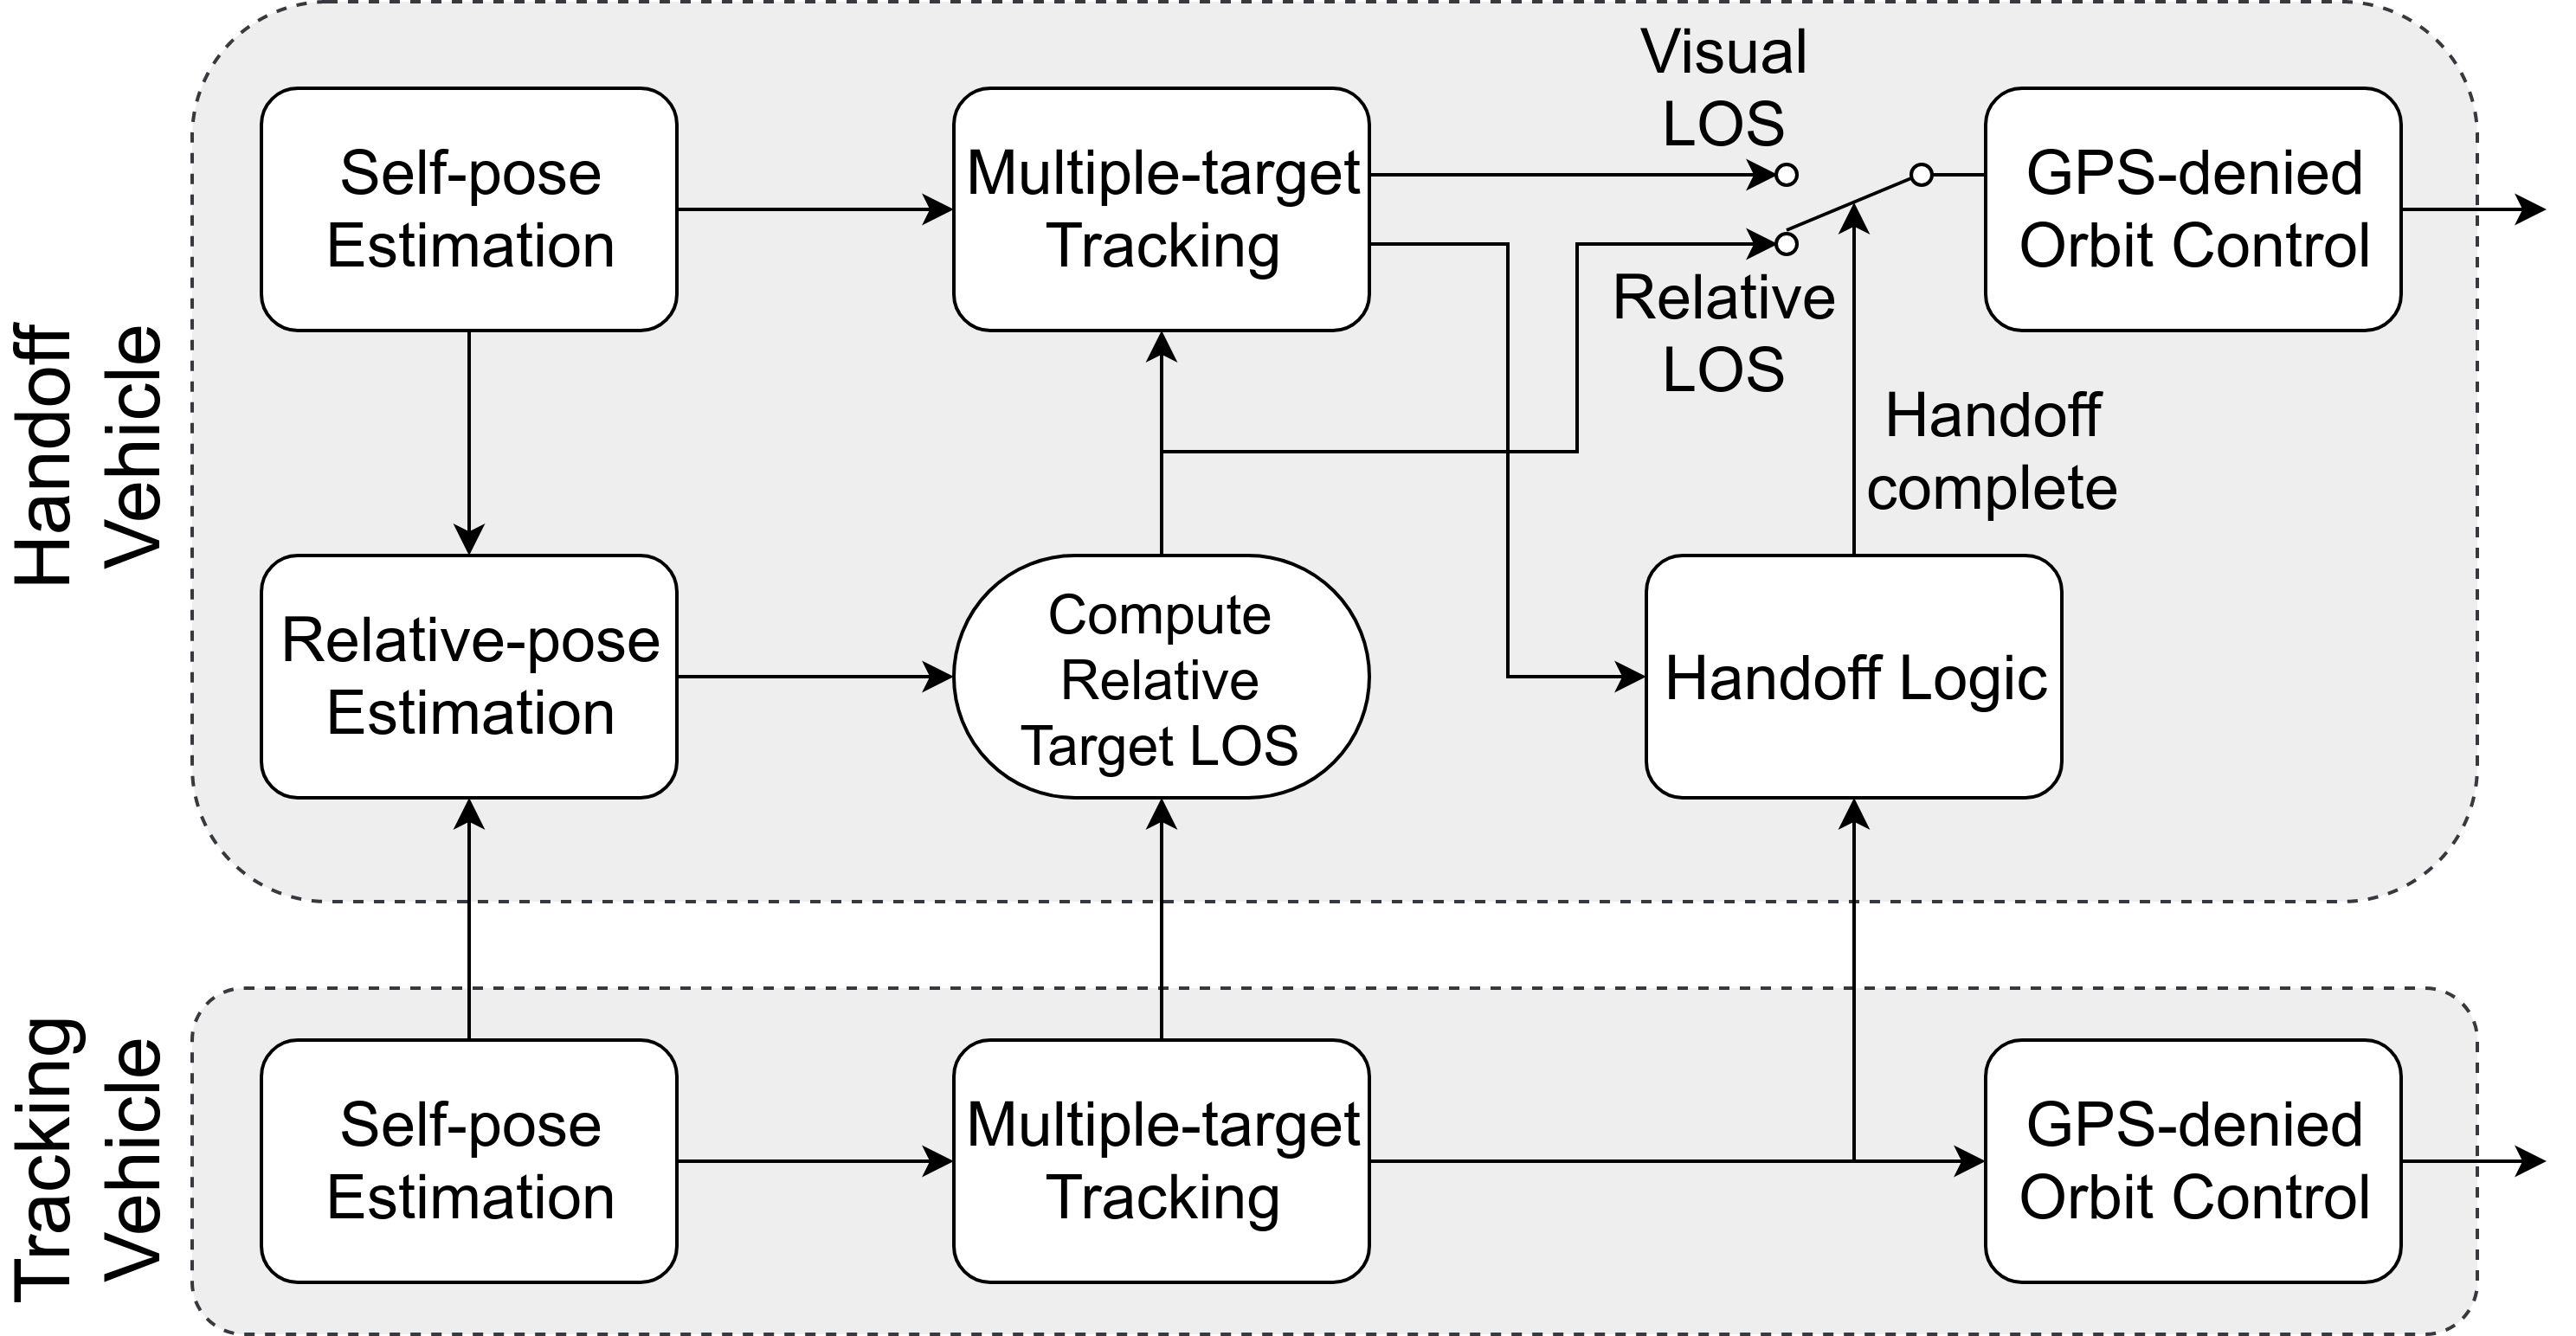
\includegraphics[width=1.0\textwidth]{figures/intro/handoff_block}
    \caption{Block diagram of the system components and information flow.}
    \label{fig:handoff_block}
\end{figure*}


This work addresses each of these challenges using either an extension of previous work or a novel solution to the problem. 
\begin{itemize}
  \item Self-pose estimation is addressed in Chapter~\ref{ch:self_pose}, and is solved using a complementary filter on $SO(3)$. and represents an extension of~\cite{Mahony11}.
  \item The estimates from the complimentary filter are inputs to a particle filter used to estimate the relative pose. A novel relative pose particle filter is derived in Chapter~\ref{ch:relative_pose}.
  \item The challenge of inserting a UAS into an orbit without GPS is solved using a controller that produces appropriate roll commands based on an estimated line of sight vector to the target. This controller is described in Chapter~\ref{ch:orbit_control}, and represents an extension of the orbit control algorithm described in~\cite{BeardMcLain12}.  
  \item The tracking and handoff UAS both utilize the Recursive-RANSAC (R-RANSAC) algorithm to visually track ground objects. While R-RANSAC was originally introduced in~\cite{NiedfeldtBeard14}, Chapter~\ref{ch:target_tracking} presents new results where the algorithm is used on a fixed-wing vehicle with a gimballed camera.
  \item Chapter~\ref{ch:handoff_logic} describes the algorithm used to perform the handoff logic, completing the moving target handoff problem.
  \item Chapter~\ref{ch:results} gives simulation results followed by some concluding remarks in Chapter~\ref{ch:conclusion}.
\end{itemize}
